%%%%%%%%%%%%%%%%%%%%%%%%%%%%%%%%%%%%%%%%%%%%%%%%%%%
%
%  New template code for TAMU Theses and Dissertations starting Fall 2012.  
%  For more info about this template or the 
%  TAMU LaTeX User's Group, see http://www.howdy.me/.
%
%  Author: Wendy Lynn Turner 
%
%%%%%%%%%%%%%%%%%%%%%%%%%%%%%%%%%%%%%%%%%%%%%%%%%%%

\documentclass[12pt]{report}
\usepackage[letterpaper]{geometry}
\geometry{verbose,tmargin=1.25in,bmargin=1.25in,lmargin=1.4in,rmargin=1.15in}
 \usepackage[doublespacing]{setspace}
 \usepackage{tocloft}
 \usepackage[rm, tiny,center, compact]{titlesec}
 \usepackage{indentfirst}
 \usepackage{etoolbox}
\usepackage{tocvsec2}
 \usepackage[titletoc]{appendix}
 \usepackage{appendix}
 \usepackage{tamuconfig}
\usepackage{rotating}

% Added to fix issues with pdf searching in some versions of LaTeX
%\usepackage[T1]{fontenc}\usepackage{lmodern}
%%%%%%%%%%%%%%%%%%%%%%%%%%%%%

% Hyperref setup below.  You should be able to get away with using uncommenting just the first line.
%\usepackage[hidelinks]{hyperref}

% if \usepackage[hidelinks]{hyperref} doesn't work try this.
% \usepackage{hyperref}  % Hidelinks is an option that removes link visiability.  TAMU Thesis Offices prefers to not see the links. But often doesn't work.  
% 
% \hypersetup{
%     colorlinks=true,
%     linkcolor=black,
%     citecolor=black,
%     filecolor=black,
%     urlcolor=black,
% }
%%%%%%%  End of hyperref setup.  One of these two options should work, but my motto with hyperref is when in doubt, comment it out!
%%%%%%%%%  This hopefully fixes the problem with vertical spacing of section headings at the top of the page..  Commented out in 1.0.7
% \preto\section{%
% \ifnum\value{section}>0\addtocontents{toc}{\vskip-6pt}\fi
% }
% \preto\subsection{%
% \ifnum\value{subsection}=0\addtocontents{toc}{\vskip-6pt}\fi
% \ifnum\value{subsection}>0\addtocontents{toc}{\vskip-6pt}\fi
% } 
%%%%%%%%%%%%%%%%%%%%%%%%%%%%%%%%%%%%%%%%%%%%%%%%%%%%%%

\begin{document}

\renewcommand{\tamumanuscripttitle}{Type in your default title here: You may need to change the spacing if the title is too long and pushes the copyright off of the titlepage }
\renewcommand{\tamupapertype}{Dissertation}
\renewcommand{\tamufullname}{First Middle Lastname}
\renewcommand{\tamudegree}{Master of Science}
\renewcommand{\tamuchairone}{Chair Name}
% Uncomment out the next line if you have co-chairs.  You will also need to edit the titlepage.tex file.
%\newcommand{\tamuchairtwo}{Additional Chair Name}
\renewcommand{\tamumemberone}{Committee Member1}
\newcommand{\tamumembertwo}{Committee Member2}
\newcommand{\tamumemberthree}{Committee Member3}
\renewcommand{\tamudepthead}{Head of Department}
\renewcommand{\tamugradmonth}{August}
\renewcommand{\tamugradyear}{2016}
\renewcommand{\tamudepartment}{Department Name}


%%%%%%%%%%%%%%%%%%%%%%%%%%%%%%%%%%%%%%%%%%%%%%%%%%%
%
%  New template code for TAMU Theses and Dissertations starting Fall 2012.  
%  For more info about this template or the 
%  TAMU LaTeX User's Group, see http://www.howdy.me/.
%
%  Author: Wendy Lynn Turner 
%	 Version 1.0 
%  Last updated 8/5/2012
%
%%%%%%%%%%%%%%%%%%%%%%%%%%%%%%%%%%%%%%%%%%%%%%%%%%%

%%%%%%%%%%%%%%%%%%%%%%%%%%%%%% 
%% TITLE PAGE
%% The values get updated automatically.  Please do not make changes to this file other than adding/deleting committee members where necessary.
%%%%%%%%%%%%%%%%%%%%%%%%%%%%%%

\providecommand{\tabularnewline}{\\}



\begin{titlepage}
\begin{center}
\MakeUppercase{\tamumanuscripttitle}
\vspace{4em}

A \tamupapertype

by

\MakeUppercase{\tamufullname}

\vspace{4em}

\begin{singlespace}

Submitted to the Office of Graduate and Professional Studies of \\
Texas A\&M University \\

in partial fulfillment of the requirements for the degree of \\
\end{singlespace}

\MakeUppercase{\tamudegree}
\par\end{center}
\vspace{2em}
\begin{singlespace}
\begin{tabular}{ll}
 & \tabularnewline
& \cr
% If you have Co-Chairs comment out the 'Chair of Committee' line below and uncomment the 'Co-Chairs of Committee' line.
Chair of Committee, & \tamuchairone\tabularnewline
%Co-Chairs of Committee, & \tamuchairone\tabularnewline & \tamuchairtwo\tabularnewline
Committee Members, & \tamumemberone\tabularnewline
 & \tamumembertwo\tabularnewline
 & \tamumemberthree\tabularnewline
Head of Department, & \tamudepthead\tabularnewline

\end{tabular}
\end{singlespace}
\vspace{3em}

\begin{center}
\tamugradmonth \hspace{2pt} \tamugradyear

\vspace{3em}

Major Subject: \tamudepartment \par
\vspace{3em}
Copyright \tamugradyear \hspace{.5em}\tamufullname 
\par\end{center}
\end{titlepage}
\pagebreak{}




 % This is simply a file that formats and adds your titlepage, please do not edit this unless you have a specific need. .
%%%%%%%%%%%%%%%%%%%%%%%%%%%%%%%%%%%%%%%%%%%%%%%%%%%
%
%  New template code for TAMU Theses and Dissertations starting Fall 2012.  
%  For more info about this template or the 
%  TAMU LaTeX User's Group, see http://www.howdy.me/.
%
%  Author: Wendy Lynn Turner 
%	 Version 1.0 
%  Last updated 8/5/2012
%
%%%%%%%%%%%%%%%%%%%%%%%%%%%%%%%%%%%%%%%%%%%%%%%%%%%
%%%%%%%%%%%%%%%%%%%%%%%%%%%%%%%%%%%%%%%%%%%%%%%%%%%%%%%%%%%%%%%%%%%%%
%%                           ABSTRACT 
%%%%%%%%%%%%%%%%%%%%%%%%%%%%%%%%%%%%%%%%%%%%%%%%%%%%%%%%%%%%%%%%%%%%%

\chapter*{ABSTRACT}
\addcontentsline{toc}{chapter}{ABSTRACT} % Needs to be set to part, so the TOC doesnt add 'CHAPTER ' prefix in the TOC.

\pagestyle{plain} % No headers, just page numbers
\pagenumbering{roman} % Roman numerals
\setcounter{page}{2}

\indent Lorem ipsum dolor sit amet, consectetur adipiscing elit. Integer lectus quam, condimentum quis bibendum eu, sollicitudin eget lacus. Praesent non sodales odio. Class aptent taciti sociosqu ad litora torquent per conubia nostra, per inceptos himenaeos. Nulla ac luctus sapien. Morbi cursus sapien eget lorem fermentum hendrerit. Nam ac erat dui, in cursus velit. Vivamus hendrerit porttitor nisi, ut porttitor lorem volutpat eget. In ligula ligula, euismod ut condimentum sit amet, pulvinar sit amet diam. Pellentesque interdum, ipsum ullamcorper consequat dignissim, sem arcu egestas mauris, vitae interdum sem tortor ut ante. Nunc blandit laoreet nisi, non rutrum lorem hendrerit quis. Cras nunc diam, convallis et feugiat at, auctor id libero. Nunc facilisis massa eu eros imperdiet vestibulum. Vestibulum ante ipsum primis in faucibus orci luctus et ultrices posuere cubilia Curae; Donec non velit vitae tortor blandit semper.

Etiam vitae dolor nulla. Ut eros odio, rhoncus eget placerat vitae, elementum ac ante. Proin vitae odio eu nisl pharetra mattis. Pellentesque habitant morbi tristique senectus et netus et malesuada fames ac turpis egestas. Phasellus fermentum lacus consectetur neque consequat ullamcorper. Cras blandit urna non dui consequat molestie. Curabitur viverra nibh at nisi semper faucibus. Nam egestas mauris a enim dignissim nec consectetur tortor rutrum. Mauris at nisi in est luctus congue ut mattis est. Ut pretium, mi quis elementum cursus, ante eros suscipit ligula, ut porttitor elit leo sed turpis. Nam sed dui ligula.

 

\pagebreak{}

%%%%%%%%%%%%%%%%%%%%%%%%%%%%%%%%%%%%%%%%%%%%%%%%%%%
%
%  New template code for TAMU Theses and Dissertations starting Fall 2012.  
%  For more info about this template or the 
%  TAMU LaTeX User's Group, see http://www.howdy.me/.
%
%  Author: Wendy Lynn Turner 
%	 Version 1.0 
%  Last updated 8/5/2012
%
%%%%%%%%%%%%%%%%%%%%%%%%%%%%%%%%%%%%%%%%%%%%%%%%%%%

%%%%%%%%%%%%%%%%%%%%%%%%%%%%%%%%%%%%%%%%%%%%%%%%%%%%%%%%%%%%%%%%%%%%%%
%%                           DEDICATION
%%%%%%%%%%%%%%%%%%%%%%%%%%%%%%%%%%%%%%%%%%%%%%%%%%%%%%%%%%%%%%%%%%%%%
\chapter*{DEDICATION}
\addcontentsline{toc}{chapter}{DEDICATION}  % Needs to be set to part, so the TOC doesnt add 'CHAPTER ' prefix in the TOC.



\indent This is an optional page.  Lorem ipsum dolor sit amet, consectetur adipiscing elit. Integer lectus quam, condimentum quis bibendum eu, sollicitudin eget lacus. Praesent non sodales odio. Class aptent taciti sociosqu ad litora torquent per conubia nostra, per inceptos himenaeos. Nulla ac luctus sapien. Morbi cursus sapien eget lorem fermentum hendrerit. Nam ac erat dui, in cursus velit. Vivamus hendrerit porttitor nisi, ut porttitor lorem volutpat eget. In ligula ligula, euismod ut condimentum sit amet, pulvinar sit amet diam. Pellentesque interdum, ipsum ullamcorper consequat dignissim, sem arcu egestas mauris, vitae interdum sem tortor ut ante. Nunc blandit laoreet nisi, non rutrum lorem hendrerit quis. Cras nunc diam, convallis et feugiat at, auctor id libero. Nunc facilisis massa eu eros imperdiet vestibulum. Vestibulum ante ipsum primis in faucibus orci luctus et ultrices posuere cubilia Curae; Donec non velit vitae tortor blandit semper.

Etiam vitae dolor nulla. Ut eros odio, rhoncus eget placerat vitae, elementum ac ante. Proin vitae odio eu nisl pharetra mattis. Pellentesque habitant morbi tristique senectus et netus et malesuada fames ac turpis egestas. Phasellus fermentum lacus consectetur neque consequat ullamcorper. Cras blandit urna non dui consequat molestie. Curabitur viverra nibh at nisi semper faucibus. Nam egestas mauris a enim dignissim nec consectetur tortor rutrum. Mauris at nisi in est luctus congue ut mattis est. Ut pretium, mi quis elementum cursus, ante eros suscipit ligula, ut porttitor elit leo sed turpis. Nam sed dui ligula.


\pagebreak{}

%%%%%%%%%%%%%%%%%%%%%%%%%%%%%%%%%%%%%%%%%%%%%%%%%%%
%
%  New template code for TAMU Theses and Dissertations starting Fall 2012.  
%  For more info about this template or the 
%  TAMU LaTeX User's Group, see http://www.howdy.me/.
%
%  Author: Wendy Lynn Turner 
%	 Version 1.0 
%  Last updated 8/5/2012
%
%%%%%%%%%%%%%%%%%%%%%%%%%%%%%%%%%%%%%%%%%%%%%%%%%%%


%%%%%%%%%%%%%%%%%%%%%%%%%%%%%%%%%%%%%%%%%%%%%%%%%%%%%%%%%%%%%%%%%%%%%%
%%                           ACKNOWLEDGEMENTS
%%%%%%%%%%%%%%%%%%%%%%%%%%%%%%%%%%%%%%%%%%%%%%%%%%%%%%%%%%%%%%%%%%%%%
\chapter*{ACKNOWLEDGEMENTS}
\addcontentsline{toc}{chapter}{ACKNOWLEDGEMENTS}  % Needs to be set to part, so the TOC doesnt add 'CHAPTER ' prefix in the TOC.


\indent Lorem ipsum dolor sit amet, consectetur adipiscing elit. Integer lectus quam, condimentum quis bibendum eu, sollicitudin eget lacus. Praesent non sodales odio. Class aptent taciti sociosqu ad litora torquent per conubia nostra, per inceptos himenaeos. Nulla ac luctus sapien. Morbi cursus sapien eget lorem fermentum hendrerit. Nam ac erat dui, in cursus velit. Vivamus hendrerit porttitor nisi, ut porttitor lorem volutpat eget. In ligula ligula, euismod ut condimentum sit amet, pulvinar sit amet diam. Pellentesque interdum, ipsum ullamcorper consequat dignissim, sem arcu egestas mauris, vitae interdum sem tortor ut ante. Nunc blandit laoreet nisi, non rutrum lorem hendrerit quis. Cras nunc diam, convallis et feugiat at, auctor id libero. Nunc facilisis massa eu eros imperdiet vestibulum. Vestibulum ante ipsum primis in faucibus orci luctus et ultrices posuere cubilia Curae; Donec non velit vitae tortor blandit semper.

Etiam vitae dolor nulla. Ut eros odio, rhoncus eget placerat vitae, elementum ac ante. Proin vitae odio eu nisl pharetra mattis. Pellentesque habitant morbi tristique senectus et netus et malesuada fames ac turpis egestas. Phasellus fermentum lacus consectetur neque consequat ullamcorper. Cras blandit urna non dui consequat molestie. Curabitur viverra nibh at nisi semper faucibus. Nam egestas mauris a enim dignissim nec consectetur tortor rutrum. Mauris at nisi in est luctus congue ut mattis est. Ut pretium, mi quis elementum cursus, ante eros suscipit ligula, ut porttitor elit leo sed turpis. Nam sed dui ligula.


\pagebreak{}
%%%%%%%%%%%%%%%%%%%%%%%%%%%%%%%%%%%%%%%%%%%%%%%%%%%
%
%  New template code for TAMU Theses and Dissertations starting Fall 2012.  
%  For more info about this template or the 
%  TAMU LaTeX User's Group, see http://www.howdy.me/.
%
%  Author: Wendy Lynn Turner 
%	 Version 1.0 
%  Last updated 8/5/2012
%
%%%%%%%%%%%%%%%%%%%%%%%%%%%%%%%%%%%%%%%%%%%%%%%%%%%

%%%%%%%%%%%%%%%%%%%%%%%%%%%%%%%%%%%%%%%%%%%%%%%%%%%%%%%%%%%%%%%%%%%%%%
%%                           NOMENCLATURE
%%%%%%%%%%%%%%%%%%%%%%%%%%%%%%%%%%%%%%%%%%%%%%%%%%%%%%%%%%%%%%%%%%%%%

\chapter*{NOMENCLATURE}
\addcontentsline{toc}{chapter}{NOMENCLATURE}  % Needs to be set to part, so the TOC doesnt add 'CHAPTER ' prefix in the TOC.

\begin{tabular}{ll}
B/CS  & Bryan/College Station\tabularnewline
HSUS & Humane Society of the United States\tabularnewline
P & Pressure\tabularnewline
T  & Time\tabularnewline
TVA & Tennessee Valley Authority\tabularnewline
TxDOT \hfill{}\hfill{}\hfill{}\hfill{}\hfill{}\hfill{}\hfill{}\hfill{} & \multicolumn{1}{l}{Texas Department of Transportation}\tabularnewline
\end{tabular}

\vspace{2em}

This page is optional.

\pagebreak{}

%%%%%%%%%%%%%%%%%%%%%%%%%%%%%%%%%%%%%%%%%%%%%%%%%%%
%
%  New template code for TAMU Theses and Dissertations starting Fall 2012.  
%  For more info about this template or the 
%  TAMU LaTeX User's Group, see http://www.howdy.me/.
%
%  Author: Wendy Lynn Turner 
%	 Version 1.7
%  Last updated 3/24/2014
%
%%%%%%%%%%%%%%%%%%%%%%%%%%%%%%%%%%%%%%%%%%%%%%%%%%%
%%%%%%%%%%%%%%%%%%%%%%%%%%%%%%%%%%%%%%%%%%%%%%%%%%%%%%%%%%%%%%%%%%%%%%
%%       TABLE OF CONTENTS
%%%%%%%%%%%%%%%%%%%%%%%%%%%%%%%%%%%%%%%%%%%%%%%%%%%%%%%%%%%%%%%%%%%%%
% single-space sections in Table of Contents  - commented in version 1.7
%\renewcommand{\cftsecafterpnum}{\vskip0.5\baselineskip}
%\renewcommand{\cftsubsecafterpnum}{\vskip0.5\baselineskip}
%\renewcommand{\cftsubsubsecafterpnum}{\vskip0.5\baselineskip}
%%%%%%%%%%%%%%%%%%%%%%%%%%%%%%%%%%%%%%%%%%%%%%%%%%%

\phantomsection
\addcontentsline{toc}{chapter}{TABLE OF CONTENTS}  

\begin{singlespace}
\renewcommand\contentsname{\normalfont} {\centerline{TABLE OF CONTENTS}}

%\setcounter{tocdepth}{4} % This puts \subsubsection[]{×} in your List of Tables.  The default is 3.


%%%%%%%%%%%%%  Adds Page above the page number in TOC
\setlength{\cftaftertoctitleskip}{1em}
\renewcommand{\cftaftertoctitle}{%
\hfill{\normalfont {Page}\par}}



\tableofcontents

\end{singlespace}

\pagebreak{}

%%%%%%%%%%%%%%%%%%%%%%%%%%%%%%%%%%%%%%%%%%%%%%%%%%%%%%%%%%%%%%%%%%%%%%
%%                           LIST OF FIGURES
%%%%%%%%%%%%%%%%%%%%%%%%%%%%%%%%%%%%%%%%%%%%%%%%%%%%%%%%%%%%%%%%%%%%%

\phantomsection
\addcontentsline{toc}{chapter}{LIST OF FIGURES}  

\renewcommand{\cftloftitlefont}{\center\normalfont\MakeUppercase}

\setlength{\cftbeforeloftitleskip}{-12pt} %% Positions the LOF title vertically to match the chapter titles
\renewcommand{\cftafterloftitleskip}{12pt}


\renewcommand{\cftafterloftitle}{%
\\[4em]\mbox{}\hspace{2pt}FIGURE\hfill{\normalfont Page}\vskip\baselineskip}

\begingroup


\begin{center}
\begin{singlespace}
%% These values make the lof table entries appear double spaced between.
\setlength{\cftbeforechapskip}{0.4cm}
\setlength{\cftbeforesecskip}{0.30cm}
\setlength{\cftbeforesubsecskip}{0.30cm}
\setlength{\cftbeforefigskip}{0.4cm}
\setlength{\cftbeforetabskip}{0.4cm} 

\listoffigures

\end{singlespace}
\end{center}

\pagebreak{}


%%%%%%%%%%%%%%%%%%%%%%%%%%%%%%%%%%%%%%%%%%%%%%%%%%%%%%%%%%%%%%%%%%%%%%
%%                           lIST OF TABLES
%%%%%%%%%%%%%%%%%%%%%%%%%%%%%%%%%%%%%%%%%%%%%%%%%%%%%%%%%%%%%%%%%%%%%%
%
\phantomsection
\addcontentsline{toc}{chapter}{LIST OF TABLES}  

\renewcommand{\cftlottitlefont}{\center\normalfont\MakeUppercase}

\setlength{\cftbeforelottitleskip}{-12pt} %% Positions the LOT title vertically to match the chapter titles

\renewcommand{\cftafterlottitleskip}{12pt}


\renewcommand{\cftafterlottitle}{%
\\[4em]\mbox{}\hspace{4pt}TABLE\hfill{\normalfont Page}\vskip\baselineskip}

\begin{center}
\begin{singlespace}

%% These values make the lot table entries appear double spaced between.
\setlength{\cftbeforechapskip}{0.4cm}
\setlength{\cftbeforesecskip}{0.30cm}
\setlength{\cftbeforesubsecskip}{0.30cm}
\setlength{\cftbeforefigskip}{0.4cm}
\setlength{\cftbeforetabskip}{0.4cm}

\listoftables 

\end{singlespace}
\end{center}
\endgroup
\pagebreak{}  % Need this for the pagenumbering to be correct.   % This is simply a file that formats and adds your toc, lof, and lot, please do not edit this unless you have a specific need. .

%%%%%%%%%%%%%%%%%%%%%%%%%%%%%%%%%%%%%%%%%%%%%%%%%%%
%
%  New template code for TAMU Theses and Dissertations starting Fall 2012.  
%  For more info about this template or the 
%  TAMU LaTeX User's Group, see http://www.howdy.me/.
%
%  Author: Wendy Lynn Turner 
%	 Version 1.0 
%  Last updated 8/5/2012
%
%%%%%%%%%%%%%%%%%%%%%%%%%%%%%%%%%%%%%%%%%%%%%%%%%%%

%%%%%%%%%%%%%%%%%%%%%%%%%%%%%%%%%%%%%%%%%%%%%%%%%%%%%%%%%%%%%%%%%%%%%%
%%                           SECTION I
%%%%%%%%%%%%%%%%%%%%%%%%%%%%%%%%%%%%%%%%%%%%%%%%%%%%%%%%%%%%%%%%%%%%%


\pagestyle{plain} % No headers, just page numbers
\pagenumbering{arabic} % Arabic numerals
\setcounter{page}{1}


\chapter{\uppercase {Introduction: The Importance of Research}}


Text goes here.

\section{This is a Very Long Section Title This is a Very Long Section Title This is a Very Long Section Title }

A landscape figure should be shown below. 
%%%%%%%%%%%%%%%%%%%%%%%%%%%%%%%%%%%%%%%%%%%%%%%%%%%%%%
\begin{sidewaysfigure}[H]
\centering
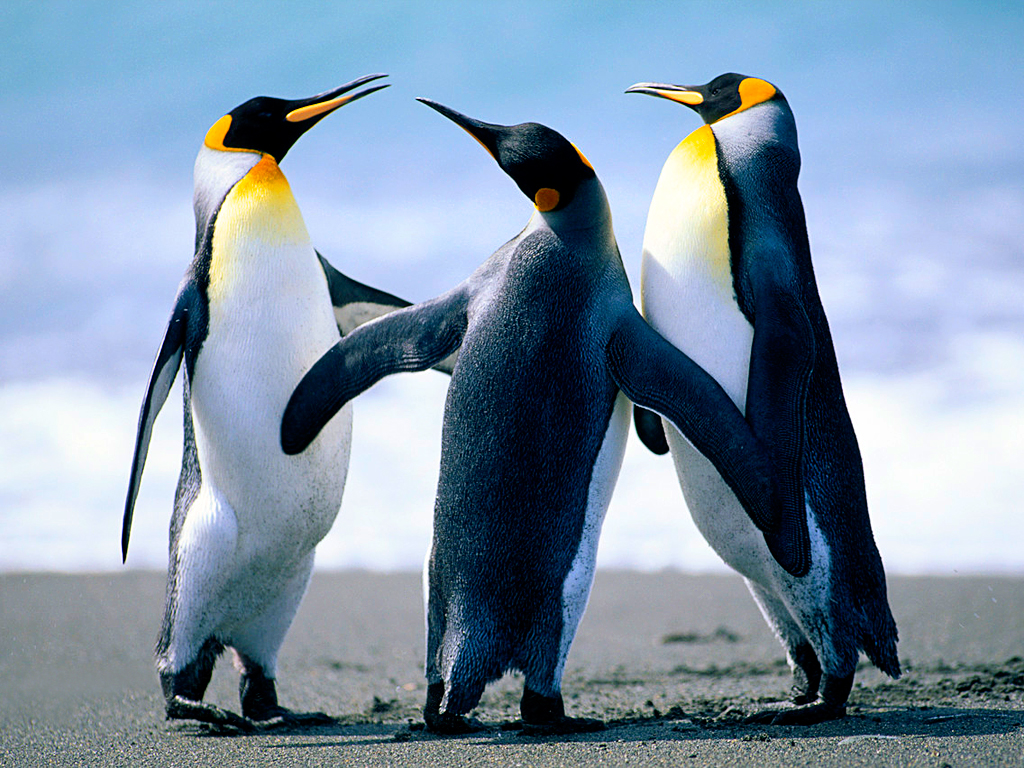
\includegraphics[scale=.50]{figures/Penguins.jpg}
\caption{TAMU figure - This is an example of a long figure title with a landscape figure.  Figure titles need to be single-spaced within and double spaced between in the list of figures.}
\label{fig:tamu-fig1-1}
\end{sidewaysfigure}
%%%%%%%%%%%%%%%%%%%%%%%%%%%%%%%%%%%%%%%%%%%%%%%%%%%%%%

More text here goes here.


Lorem ipsum dolor sit amet, consectetur adipiscing elit. Morbi augue urna, varius quis facilisis ac, imperdiet et nunc. Vestibulum ante ipsum primis in faucibus. 

\section{Testing the Top of the Page}
Maecenas accumsan lobortis dui fringilla suscipit. Quisque congue fringilla dui, sed eleifend sapien fringilla euismod. Pellentesque habitant morbi tristique senectus et netus et malesuada fames ac turpis egestas. Maecenas venenatis posuere magna quis tempus. Cras at leo massa, eu ultricies tellus. Nunc nec dictum augue. Cum sociis natoque penatibus et magnis dis parturient montes, nascetur ridiculus mus. Phasellus purus felis, mollis id scelerisque in, viverra in elit. Nulla iaculis ultrices justo, ac pharetra nisl rhoncus pulvinar. Duis vitae mauris velit, in congue massa.

Donec lectus orci, bibendum ut blandit dignissim, molestie non eros. Praesent aliquet feugiat dignissim. Morbi porttitor sollicitudin nisl, non mollis quam ultrices sit amet. Cras feugiat lacinia diam ut convallis. Nam nec varius ante. Nunc a ultrices felis. Quisque luctus sapien et ligula ornare quis consequat urna aliquet. Vestibulum vulputate lorem a tellus auctor id commodo risus sodales. Suspendisse quis tortor a felis molestie laoreet ut a nunc. Donec gravida sapien eget mauris condimentum lacinia. Proin eu purus libero. Nullam augue mi, vestibulum in convallis eu, adipiscing ac arcu. Donec nisi libero, egestas et molestie in, mollis quis ipsum. Sed gravida quam sit amet ante tempus rutrum non in mi. Cras viverra facilisis eros, id vestibulum sapien malesuada eget. Maecenas imperdiet luctus nisi vitae suscipit.



Aliquam erat volutpat. Integer ut mauris elit. Nam et lectus vel neque vehicula commodo. Integer at risus ligula. Fusce mollis mauris sed lorem aliquam bibendum porttitor tellus blandit. Curabitur enim nibh, accumsan eu elementum id, rutrum a ipsum. Vivamus ultricies, elit id ornare iaculis, metus justo posuere quam, sit amet bibendum arcu dolor a eros. Sed in nisl nibh. Aenean egestas est ut tortor volutpat vehicula. Maecenas aliquet placerat nunc hendrerit dictum. In et nisi massa. Pellentesque luctus, sapien quis dignissim vulputate, sapien libero bibendum velit, vitae auctor ipsum nulla at augue. Nulla ac eros vitae tortor elementum vehicula.

Morbi tristique egestas placerat. Cras faucibus eleifend porta. Class aptent taciti sociosqu ad litora torquent per conubia nostra, per inceptos himenaeos. Ut a pellentesque neque. Donec sollicitudin metus varius nulla egestas laoreet. Duis non mauris ut nunc adipiscing volutpat. Nam vitae est sed turpis tristique varius. 

\subsection{This is a Very Long Subsection Title This is a Very Long Subsection Title}

More text
\subsection{Subsection}

Subsection text

\section{Another Section}

Section text

%%%%%%%%%%%%%%%%%%%%%%%%%%%%%%%%%%%%%%%%%%%%%%%%%%%
%
%  New template code for TAMU Theses and Dissertations starting Fall 2012.  
%  For more info about this template or the 
%  TAMU LaTeX User's Group, see http://www.howdy.me/.
%
%  Author: Wendy Lynn Turner 
%	 Version 1.0 
%  Last updated 8/5/2012
%
%%%%%%%%%%%%%%%%%%%%%%%%%%%%%%%%%%%%%%%%%%%%%%%%%%%

%%%%%%%%%%%%%%%%%%%%%%%%%%%%%%%%%%%%%%%%%%%%%%%%%%%%%%%%%%%%%%%%%%%%%%%
%%%                           SECTION II
%%%%%%%%%%%%%%%%%%%%%%%%%%%%%%%%%%%%%%%%%%%%%%%%%%%%%%%%%%%%%%%%%%%%%%

\chapter{\uppercase {Literature Review: The Importance of Research Part Two- This is designed to test long titles in the TOC}}

Text goes here.

\section{New Section}
%%%%%%%%%%%%%%%%%%%%%%%%%%%%%%%%%%%%%%%%%%%%%%%%%%%%%%
\begin{figure}[H]
\centering

\includegraphics[scale=.50]{Figures/TAM-Logo.png}
\caption{TAMU figure - This is an example of a long figure title.  Figure titles need to be single-spaced within and double spaced between in the list of figures.}
\label{fig:landscapepenguins}
\end{figure}
%%%%%%%%%%%%%%%%%%%%%%%%%%%%%%%%%%%%%%%%%%%%%%%%%%%%%%
\subsection{Subsection}
\begin{table}[H]
\centering
\caption{This is a table template - This is an example of a long table title.  Table titles need to be single-spaced within and double spaced between in the list of tables.}
\begin{tabular}{|l|c|c|c|c|c|}
\hline
Product & 1 & 2 & 3 & 4 & 5\\
\hline
Price & 124.- & 136.- & 85.- & 156.- & 23.-\\
Guarantee [years] & 1 & 2 & - & 3 & 1\\
Rating & 89\% & 84\% & 51\% & & 45\%\\
\hline
\hline
Recommended & yes & yes & no & no & no\\
\hline
\end{tabular}
\label{tab:template1}
\end{table}


\subsection{Subsection}
%%%%%%%%%%%%%%%%%%%%%%%%%%%%%%%%%%%%%%%%%%%%%%%%%%%%%%
\begin{figure}[H]
\centering

\includegraphics[scale=.50]{Figures/TAMLogoBox.png}
\caption{Sunset figure}
\label{fig:sunset-fig2}
\end{figure}
%%%%%%%%%%%%%%%%%%%%%%%%%%%%%%%%%%%%%%%%%%%%%%%%%%%%%%
\subsubsection{This is a subsubsection}
\begin{table}[H]
\centering
\caption{This is a table template - This is an example of a long table title.  Table titles need to be single-spaced within and double spaced between in the list of tables.}
\begin{tabular}{|l|c|c|c|c|c|}
\hline
Product & 1 & 2 & 3 & 4 & 5\\
\hline
Price & 124.- & 136.- & 85.- & 156.- & 23.-\\
Guarantee [years] & 1 & 2 & - & 3 & 1\\
Rating & 89\% & 84\% & 51\% & & 45\%\\
\hline
\hline
Recommended & yes & yes & no & no & no\\
\hline
\end{tabular}
\label{tab:template1-2}
\end{table}
\section{Another Section}

%%%%%%%%%%%%%%%%%%%%%%%%%%%%%%%%%%%%%%%%%%%%%%%%%%%
%
%  New template code for TAMU Theses and Dissertations starting Fall 2012.  
%  For more info about this template or the 
%  TAMU LaTeX User's Group, see http://www.howdy.me/.
%
%  Author: Wendy Lynn Turner 
%	 Version 1.0 
%  Last updated 8/5/2012
%
%%%%%%%%%%%%%%%%%%%%%%%%%%%%%%%%%%%%%%%%%%%%%%%%%%%
%%%%%%%%%%%%%%%%%%%%%%%%%%%%%%%%%%%%%%%%%%%%%%%%%%%%%%%%%%%%%%%%%%%%%%
%%                           SECTION III
%%%%%%%%%%%%%%%%%%%%%%%%%%%%%%%%%%%%%%%%%%%%%%%%%%%%%%%%%%%%%%%%%%%%%



\chapter{\uppercase{Last Chapter: The Importance of Research}}

Text goes here \cite{Agrawal1986}.

\section{New Section}

%%%%%%%%%%%%%%%%%%%%%%%%%%%%%%%%%%%%%%%%%%%%%%%%%%%%%%
\begin{figure}[H]
\centering

\includegraphics[scale=.50]{Figures/TAM-Logo.png}
\caption{TAMU figure}
\label{fig:tamu-fig3}
\end{figure}
%%%%%%%%%%%%%%%%%%%%%%%%%%%%%%%%%%%%%%%%%%%%%%%%%%%%%%
\section{Another Section}

Text between the figures.  Text between the figures. Text between the figures. Text between the figures.  Text between the figures. Text between the figures. Text between the figures.  Text between the figures. Text between the figures. Text between the figures.  Text between the figures. Text between the figures.
%%%%%%%%%%%%%%%%%%%%%%%%%%%%%%%%%%%%%%%%%%%%%%%%%%%%%%%
%\begin{figure}[H]
%\centering
%
\includegraphics[scale=.50]{Figures/TAM-Logo.png}
%\caption{Another TAMU figure}
%\label{fig:tamu-fig4}
%\end{figure}
%%%%%%%%%%%%%%%%%%%%%%%%%%%%%%%%%%%%%%%%%%%%%%%%%%%%%%%

\subsection{Subsection}

%%%%%%%%%%%%%%%%%%%%%%%%%%%%%%%%%%%%%%%%%%%%%%%%%%%%%%%
%\begin{figure}[H]
%\centering
%
\includegraphics[scale=.50]{Figures/TAM-Logo.png}
%\caption{Another TAMU figure}
%\label{fig:tamu-fig4-2}
%\end{figure}
%%%%%%%%%%%%%%%%%%%%%%%%%%%%%%%%%%%%%%%%%%%%%%%%%%%%%%%
\subsection{Subsection}

A table example is going to follow.

\begin{table}[H]
\centering
\caption{This is a table template}
\begin{tabular}{|l|c|c|c|c|c|}
\hline
Product & 1 & 2 & 3 & 4 & 5\\
\hline
Price & 124.- & 136.- & 85.- & 156.- & 23.-\\
Guarantee [years] & 1 & 2 & - & 3 & 1\\
Rating & 89\% & 84\% & 51\% & & 45\%\\
\hline
\hline
Recommended & yes & yes & no & no & no\\
\hline
\end{tabular}
\label{tab:template2}
\end{table}
\subsubsection{This is a subsubsection}
\section{Another Section}


fix spacing in bibliography, if any...
%%%%%%%%%%%%%%%%%%%%%%%%%%%%%%%%%%%%%%%%%%%%%%%%%%%%%%%%%%%%%
\let\oldbibitem\bibitem
\renewcommand{\bibitem}{\setlength{\itemsep}{0pt}\oldbibitem}
%%%%%%%%%%%%%%%%%%%%%%%%%%%%%%%%%%%%%%%%%%%%%%%%%%%%%%%%%%%%%%%
%%%%%%%%%%%%%%%%%%%%%%%%%%%%%%%%%%%%%%%%%%%%%%%%%%%
%
%  New template code for TAMU Theses and Dissertations starting Fall 2012.  
%  For more info about this template or the 
%  TAMU LaTeX User's Group, see http://www.howdy.me/.
%
%  Author: Wendy Lynn Turner 
%	 Version 1.0 
%  Last updated 8/5/2012
%
%%%%%%%%%%%%%%%%%%%%%%%%%%%%%%%%%%%%%%%%%%%%%%%%%%%


%%%%%%%%%%%%%%%%%%%%%%%%%%%%%%%%%%%%%%%%%%%%%%%%%%%%%%%%%%%%%%%%%%%%%%
%%                           REFERENCES 
%%%%%%%%%%%%%%%%%%%%%%%%%%%%%%%%%%%%%%%%%%%%%%%%%%%%%%%%%%%%%%%%%%%%%

\phantomsection
\addcontentsline{toc}{chapter}{REFERENCES}

\renewcommand{\bibname}{{\normalsize\rm REFERENCES}}

\bibliographystyle{plain}
\bibliography{references}
% %%%%%%%%%%%%%%%%%%%%%%%%%%%%%%%%%%%%%%%%%%%%%%%%%%%
%
%  New template code for TAMU Theses and Dissertations starting Fall 2012.  
%  For more info about this template or the 
%  TAMU LaTeX User's Group, see http://www.howdy.me/.
%
%  Author: Wendy Lynn Turner 
%	 Version 1.0 
%  Last updated 8/5/2012
%
%%%%%%%%%%%%%%%%%%%%%%%%%%%%%%%%%%%%%%%%%%%%%%%%%%%

\begin{appendices}
\titleformat{\chapter}{\centering\normalsize}{APPENDIX \thechapter}{0em}{\vskip .5\baselineskip\centering}
\renewcommand{\appendixname}{APPENDIX}

%%%%%%%%%%%%%%%%%%%%%%%%%%%%%%%%%%%%%%%%%%%%%%%%%%%
%
%  New template code for TAMU Theses and Dissertations starting Fall 2012.  
%  For more info about this template or the 
%  TAMU LaTeX User's Group, see http://www.howdy.me/.
%
%  Author: Wendy Lynn Turner 
%	 Version 1.0 
%  Last updated 8/5/2012
%
%%%%%%%%%%%%%%%%%%%%%%%%%%%%%%%%%%%%%%%%%%%%%%%%%%%

%%%%%%%%%%%%%%%%%%%%%%%%%%%%%%%%%%%%%%%%%%%%%%%%%%%%%%%%%%%%%%%%%%%%%%
%%                           APPENDIX A 
%%%%%%%%%%%%%%%%%%%%%%%%%%%%%%%%%%%%%%%%%%%%%%%%%%%%%%%%%%%%%%%%%%%%%

\phantomsection

\chapter{\uppercase{First Appendix}}

Text for the Appendix follows.

\begin{figure}[H]
\centering
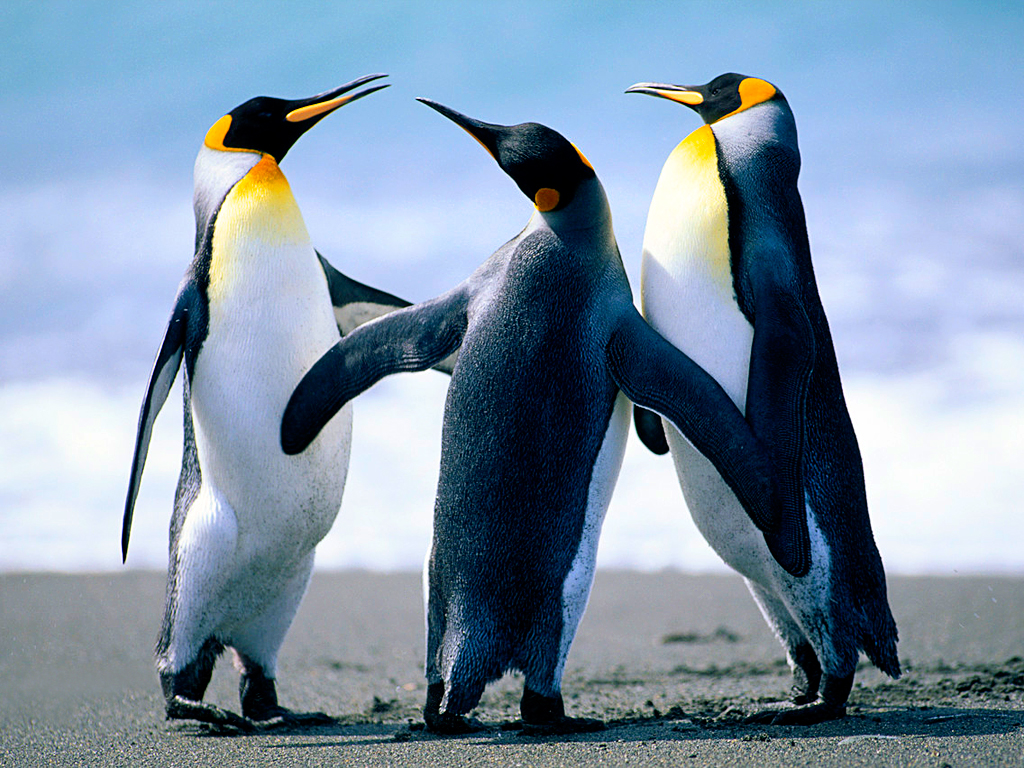
\includegraphics[scale=.50]{figures/Penguins.jpg}
\caption{TAMU figure}
\label{fig:tamu-fig5}
\end{figure}

%%%%%%%%%%%%%%%%%%%%%%%%%%%%%%%%%%%%%%%%%%%%%%%%%%%
%
%  New template code for TAMU Theses and Dissertations starting Fall 2012.  
%  For more info about this template or the 
%  TAMU LaTeX User's Group, see http://www.howdy.me/.
%
%  Author: Wendy Lynn Turner 
%	 Version 1.0 
%  Last updated 8/5/2012
%
%%%%%%%%%%%%%%%%%%%%%%%%%%%%%%%%%%%%%%%%%%%%%%%%%%%

%%%%%%%%%%%%%%%%%%%%%%%%%%%%%%%%%%%%%%%%%%%%%%%%%%%%%%%%%%%%%%%%%%%%%%
%%                           APPENDIX B
%%%%%%%%%%%%%%%%%%%%%%%%%%%%%%%%%%%%%%%%%%%%%%%%%%%%%%%%%%%%%%%%%%%%%

\chapter{\uppercase {Second Appendix with a longer title - much longer in fact}}

Text for the Appendix follows.

\begin{figure}[H]
\centering

\includegraphics[scale=.50]{Figures/TAM-Logo.png}
\caption{TAMU figure}
\label{fig:tamu-fig6}
\end{figure}

\section{Appendix Section}


\pagebreak{}


\end{appendices}


\end{document}
